\begin{boiboiboite}
	\propair
	%\propgaz
	\isentropiques
	\isothermes
\end{boiboiboite}

% idea: aircraft tyre deflation after MERTO

\subsubsection{Air dans un réservoir}

	Une masse de~\SI{5}{\kilogram} d’air est enclose dans un réservoir de~\SI{2}{\metre\cubed}. 

	\begin{enumerate}
		\item Quelles sont sa masse volumique et son volume spécifique ?
		\item Quelle est la pression si la température est de~\SI{20}{\degreeCelsius} ?
	\end{enumerate}


\subsubsection{Évolutions complexes d’un gaz parfait}

	De l’air dans un compartiment flexible est à pression de~\SI{3}{\bar}. Son énergie interne est de~\SI{836}{\kilo\joule\per\kilogram}.
	
	Il est chauffé à pression constante jusqu’à~\SI{900}{\degreeCelsius} ; il est ensuite refroidi et détendu selon $p v^{\num{1.1}} = \text{cste.}$ jusqu’à ce que sa température atteigne \SI{25}{\degreeCelsius}.

	\textit{[Question piège]} Combien d’énergie a-t-il reçu ou perdu depuis le début de l’évolution ?

\subsubsection{Pompe à air}

	Une pompe à air comprime de l’air en régime permanent, de façon adiabatique. L’air voit sa température augmenter depuis \SI{15}{\degreeCelsius} vers \SI{100}{\degreeCelsius}.\nopagebreak
	
	Quelle est la puissance spécifique consommée ?

\subsubsection{Réservoir d’air}
		\wherefrom{dérivé du rattrapage S1 2013}
		% reconstruit à partir du rattrapage 20130621

	Un réservoir hermétique d’air comprimé en béton a un volume fixe de \SI{1,2}{\metre\cubed}. L’air y est stocké à pression de \SI{2}{\bar}. \\
	Le réservoir est placé au soleil et le réchauffement solaire provoque une augmentation de température depuis \SI{5}{\degreeCelsius} vers \SI{60}{\degreeCelsius}.
	
	\begin{enumerate}
		\item Quelles sont la masse, le volume spécifique, la masse volumique et la pression à l’intérieur du réservoir, avant et après le réchauffage ?
	\end{enumerate}

	Une fois la température finale atteinte, on laisse de l’air s’échapper pour faire redescendre la pression dans le réservoir jusqu’à la pression initiale de \SI{2}{\bar}. Pendant l’échappement, la température de l’air dans le réservoir reste constante.

	\begin{enumerate}
		\shift{1}
		\item Quelle masse d’air faudrait-il laisser échapper ?
	\end{enumerate}

	On referme la soupape d’échappement et le réservoir, de nouveau hermétique, se refroidit lentement à volume constant. La température finale revient à \SI{5}{\degreeCelsius}.
	
	\begin{enumerate}
		\shift{2}
		\item Quelle est la pression finale dans le réservoir ?
	\end{enumerate}


\subsubsection{Turbine de turboréacteur}

	\wherefrom{[DS n°2 2011, 3pts]}
	
	Un/e étudiant/e démonte le turboréacteur de son Fouga Magister pour en étudier et en modifier le fonctionnement.

	Il/elle fait désormais fonctionner son moteur sur banc d’essai.
	
	À l’entrée de la turbine, les conditions sont mesurées à~\SI{110}{\metre\per\second} et~\SI{1000 }{\degreeCelsius} .
	À la sortie de la turbine, ces propriétés sont mesurées à~\SI{125}{\metre\per\second} et~\SI{650}{\degreeCelsius} .
	
	L’étudiant/e mesure que la turbine perd de la chaleur avec une puissance spécifique de~\SI{75}{\kilo\joule\per\kilogram}.
	
	\begin{enumerate}
		\item Quelle est la puissance mécanique spécifique développée par la turbine ?
		\item Quelle condition l’étudiant/e doit-il/elle maintenir pour obtenir une puissance de~\SI{1}{\mega\watt} ?
	\end{enumerate}


\subsubsection{Évolutions élémentaires : Compression isotherme}

	\wherefrom{[DS n°2 2011, 4pts]}

	Une masse de~\SI{3,5}{\kilogram} d’air est comprimée de façon réversible isotherme (à température constante) depuis \SI{2}{\bar} et~\SI{15}{\degreeCelsius} jusqu’à~\SI{45}{\bar}.
	
	\begin{enumerate}
		\item Tracez qualitativement l’évolution sur un diagramme pression-volume.
		\item Quelles sont les quantités de travail et de chaleur mises en jeu ?
		\item Si la compression était effectuée de façon adiabatique réversible, le volume final serait-il modifié ?
	\end{enumerate}
	
	
\subsubsection{Évolutions élémentaires : Réservoir déformable}

	\wherefrom{[DS n°2 2010, 5pts]}

	Une masse de~\SI{2}{\kilogram} d’air dans un réservoir déformable est à pression de~\SI{4,5}{\bar} et occupe un volume de~\SI{800}{\liter}. Elle est refroidie et le réservoir maintient la pression constante jusqu’à ce que le volume ait été réduit de~\SI{40}{\percent}.
	
	Ensuite, le refroidissement est continué à volume constant jusqu’à ce que la température atteigne \SI{25}{\degreeCelsius}.
	
	\begin{enumerate}
		\item Tracez l’évolution suivie sur un diagramme pression-volume.
		\item Quel est le travail effectué par l’air ?
		\item Quel est le coût total en chaleur pour l’entièreté de l’évolution ?
	\end{enumerate}


\subsubsection{Exercice bête et méchant de vocabulaire}

	\wherefrom{[DS n°2 2010, 2pts]}

	Une masse fixe de gaz parfait suit les évolutions réversibles suivantes :

		\begin{center}
			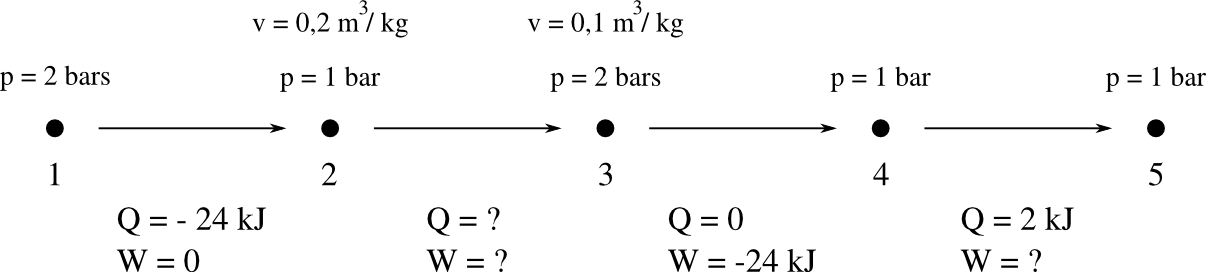
\includegraphics[width=\textwidth]{images/exo.png}
		\end{center}

	Parmi les évolutions ci-dessus, identifiez la ou les évolution(s) : 
	\begin{itemize}
		\item à température constante (isotherme) ;
		\item à volume constant (isochore).
	\end{itemize}


\subsubsection{Évolutions élémentaires d’un gaz parfait}

	\wherefrom{Partiel S1 2013, 2pts}
	
	\begin{figure}
		\begin{center}
			\vspace{-0.1cm}%handmade
			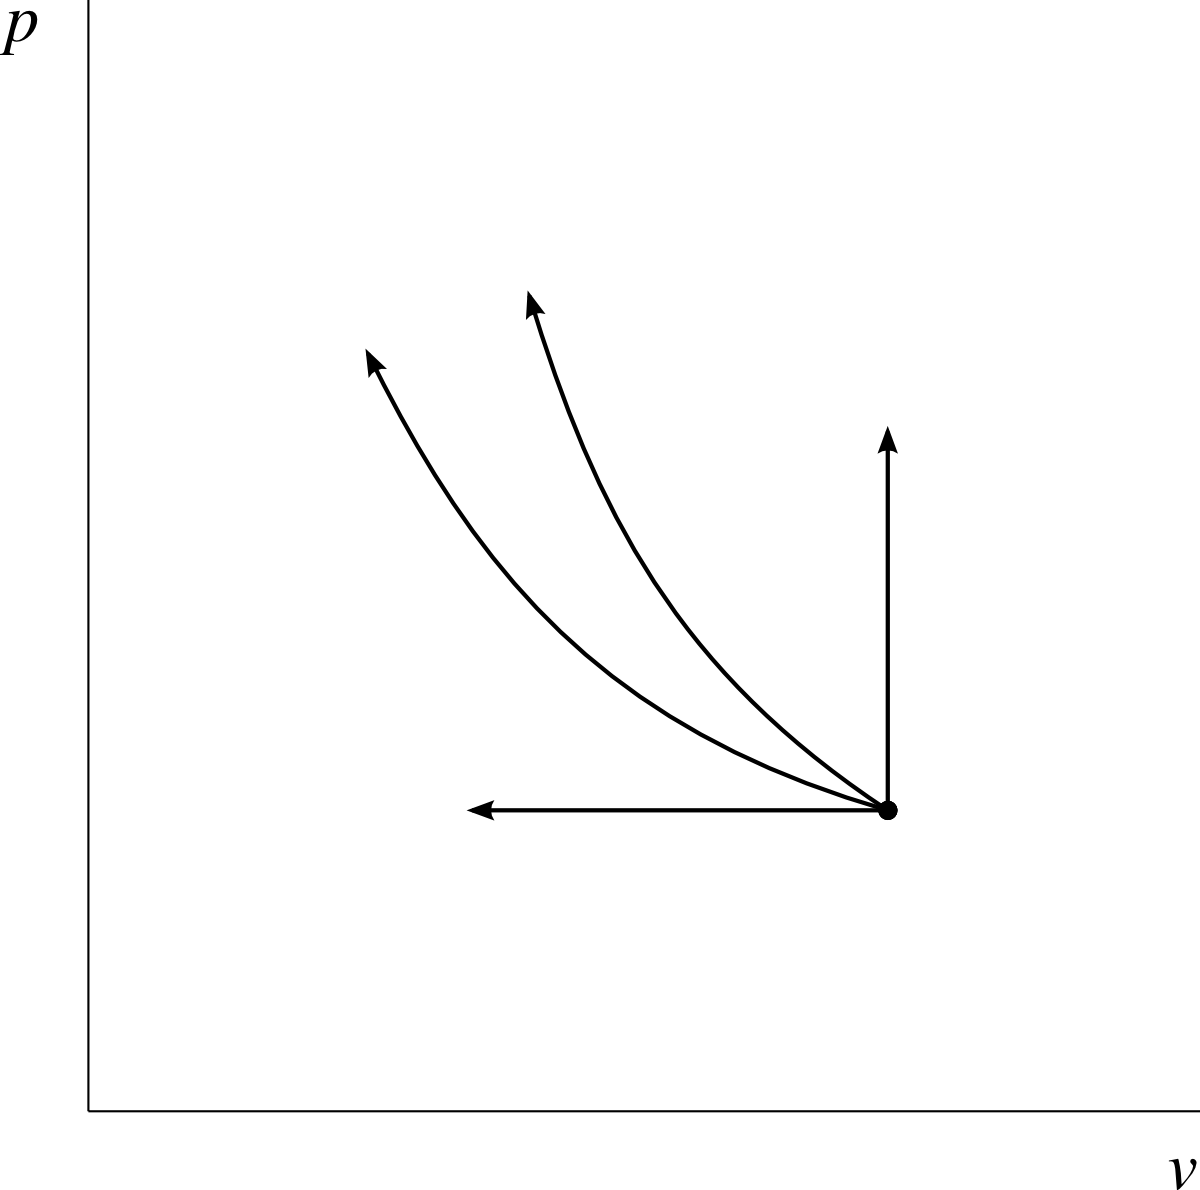
\includegraphics[width=0.4\textwidth]{images/pvel1.png}
			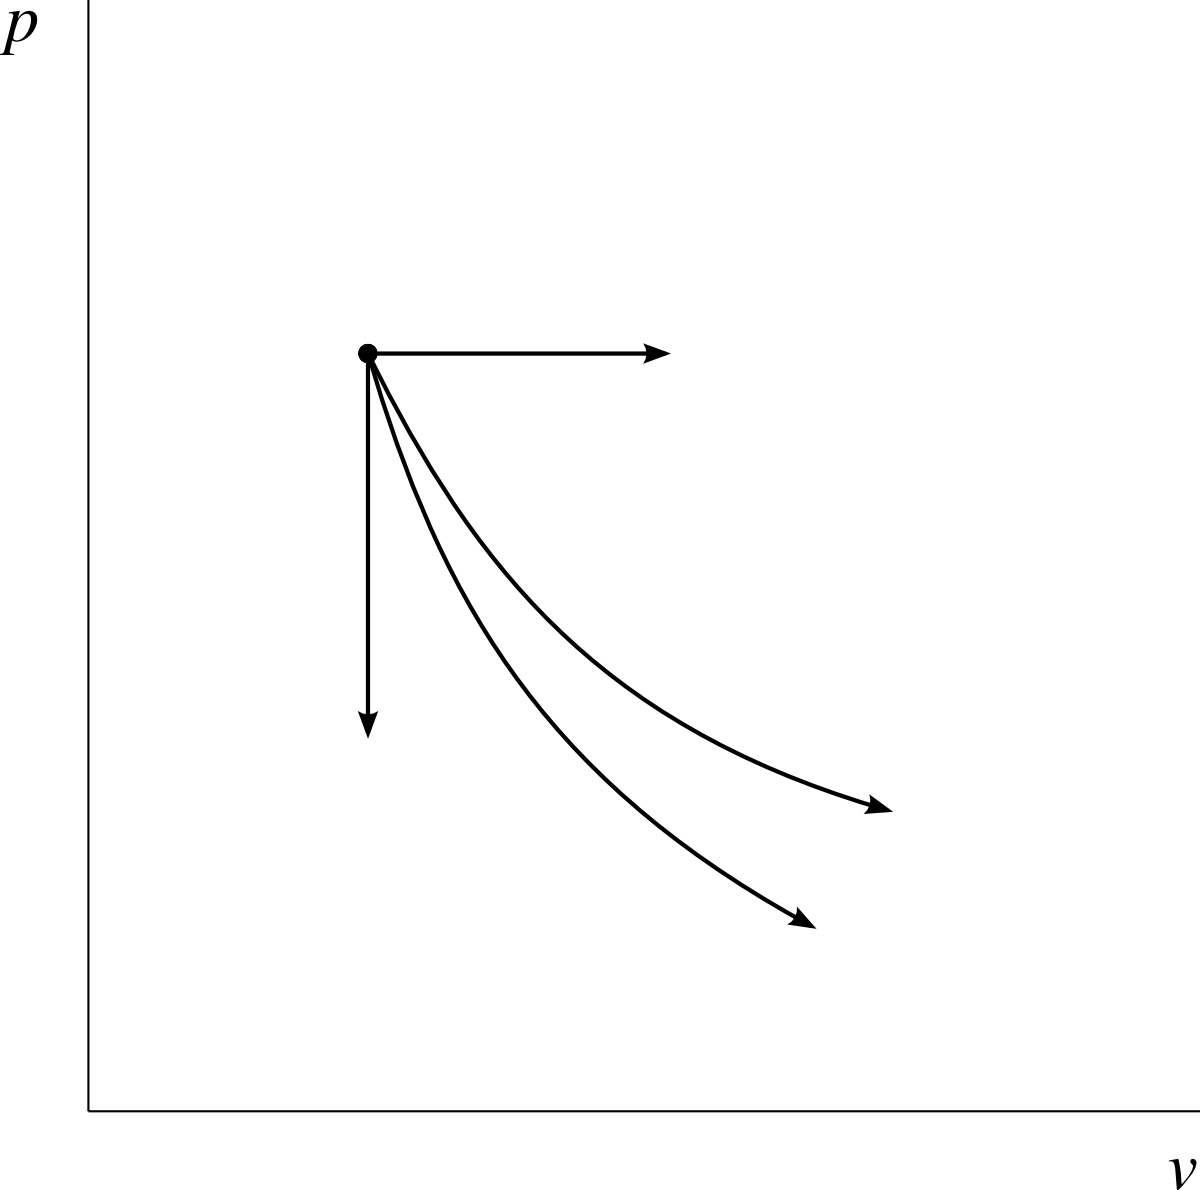
\includegraphics[width=0.4\textwidth]{images/pvel2.png}
			\vspace{-0.1cm}%handmade
		\end{center}
		\caption{Évolutions élémentaires d’un gaz parfait}
		\label{fig_pvel}
	\end{figure}

	Parmi les évolutions décrites en \cref{fig_pvel}, identifiez l’évolution à température constante, à pression constante, adiabatique réversible, et à volume constant. Aucune justification n’est demandée.


\subsubsection{Compression et combustion au sein d’un moteur Diesel}

	\wherefrom{[Partiel S1 2012, 8pts]}

	En 1890 un jeune ingénieur allemand épris de thermodynamique met au point un moteur de faible puissance, faible vitesse et haute efficacité dans un laboratoire (\cref{fig_exo_diesel}). Le moteur n’a qu’un cylindre\footnote{Mais cela ne l’empêchera pas de conquérir le monde…}. Nous étudions ici une partie de son cycle de fonctionnement. %why not more?	
	\begin{figure}
		\begin{center}
			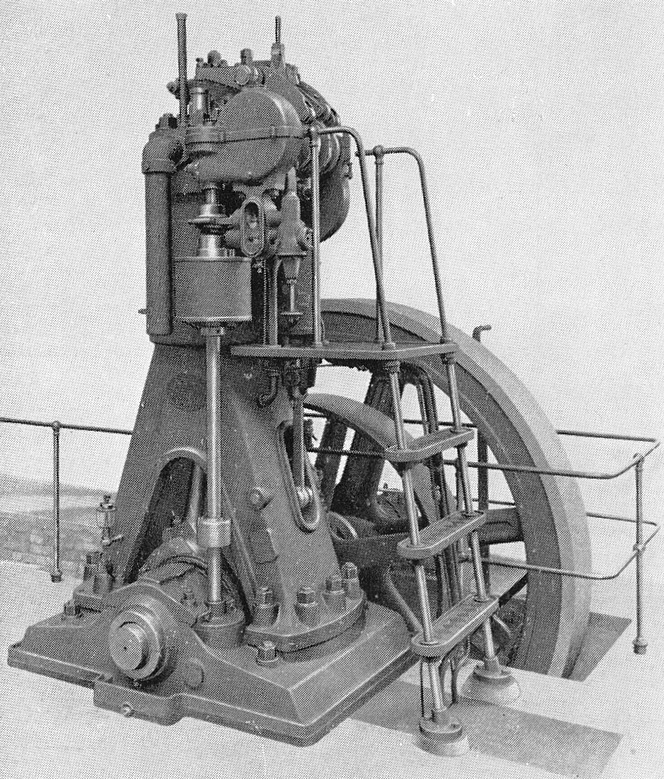
\includegraphics[width=0.5\textwidth]{images/Dieselmotor_1898_retouched.jpg}
		\end{center}
		\supercaption{Moteur Diesel de 1898, fabriqué sous licence par Sulzer en Suisse}{\wcfile{Dieselmotor 1898 (retouched).jpg}{Photo} \ccbysa Sulzer AG}
		\label{fig_exo_diesel}
	\end{figure}
	
	Le piston au sein du cylindre fait varier périodiquement le volume entre \SI{3}{\liter} (\textit{point mort bas}, piston en bas de sa course) et~\SI{0,3}{\liter} (\textit{point mort haut}, piston en haut de sa course).
	
	Le moteur débute son cycle au point mort bas, alors qu’il est empli d’air à~\SI{20}{\degreeCelsius} et~\SI{1}{\bar}. Le piston comprime cet air jusqu’au point mort haut.
	
	La compression se fait de façon réversible (très lente), mais non-adiabatique : l’air reçoit de la chaleur au travers des parois tout au long de l’évolution. L’ingénieur prédit que ses propriétés varieront selon la relation $p v^{1,5} = \text{cste.}$.


	\begin{enumerate}
		\item À partir de la définition du travail,
			\begin{equation}
				W_{F/l} \equiv \vec F \cdot \vec l 		\tag{\ref{eq_travail_fdl}}
			\end{equation}
			exprimez le travail effectué sur un corps de masse fixe en fonction de son volume spécifique et de sa pression interne.
		\item Combien d’énergie sous forme de travail la compression du gaz aura-t-elle coûté ?
		\item Combien d’énergie sous forme de chaleur le gaz aura-t-il reçu pendant la compression ?
	\end{enumerate}

	Lorsque le piston est arrivé en haut de sa course, on procède à l’injection progressive de carburant dans le cylindre pour permettre la combustion. La quantité de carburant injectée permet un apport total de chaleur de~\SI{2}{\kilo\joule}. La combustion se déroule à pression constante.
	
	\begin{enumerate}
		\shift{3}
		\item Tracez qualitativement l’évolution suivie par le gaz pendant la compression et la combustion sur un diagramme pression-volume.
		\item Quelle sera la température maximale atteinte au sein du moteur ?
		\item Pour éviter une défaillance structurelle, l’ingénieur doit s’assurer que la force transmise par le piston n’excède pas \SI{10}{\kilo\newton}. Quelle contrainte doit-il respecter pour cela ?
	\end{enumerate}



\subsubsection{Compresseur de turboréacteur}

	\wherefrom{[Partiel S1 2012, 8pts]}

	À l’intérieur d’un des moteurs d’un petit avion de ligne, le compresseur (\cref{fig_exo_compresseur_turbojet}) est approximativement adiabatique.	
	\begin{figure}
		\begin{center}
			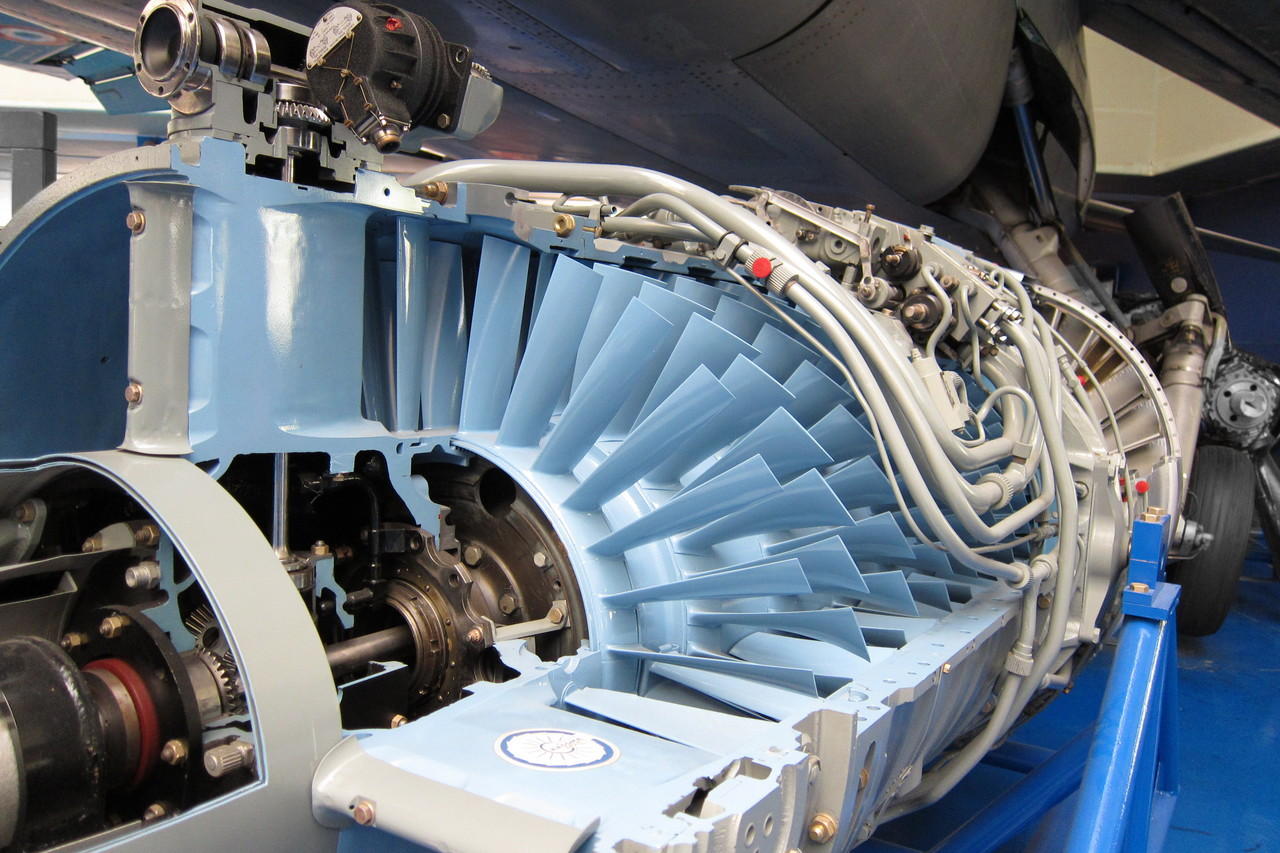
\includegraphics[width=0.8\textwidth]{images/atar_compressor.jpg}
		\end{center}
		\supercaption{Compresseur d’un turboréacteur simple flux \wfd{Snecma Atar}{\textsc{snecma} Atar} (1948) découpé. L’air s’écoule depuis le coin gauche vers le centre de l’image.}{\wcfile{Compressor of Atar turbojet.jpg}{Photo} \ccbysa \olivier}
		\label{fig_exo_compresseur_turbojet}
	\end{figure}
	
	Pendant la croisière (atmosphère : \SI{33 000}{ft} ; \SI{-50}{\degreeCelsius} ; \SI{0,25}{\bar}), le compresseur est entraîné par la turbine par le biais d’un arbre mécanique. Il reçoit \SI{7}{\kilogram\per\second} d’air aux conditions atmosphériques, qu’il compresse jusqu’à une pression de~\SI{8}{\bar}.
	
	\begin{enumerate}
		\item À partir de la relation suivante,
			\begin{equation}
				\left( \frac{p_1}{p_2} \right)	= \left( \frac{v_2}{v_1} \right)^{\gamma} \tag{\ref{eq_isentropique_horrible3}}
			\end{equation}
							
			valable pour une évolution adiabatique réversible d’un gaz parfait, montrez (sans utiliser l’\cref{eq_isentropique_horrible1}) que :
			
			\begin{equation}
				\left( \frac{T_1}{T_2} \right)	=  \left( \frac{p_1}{p_2} \right)^{\frac{\gamma -1}{\gamma}}  \tag{\ref{eq_isentropique_horrible2}}
			\end{equation}
			
		\item Quelle est la puissance minimale théorique que la turbine doit fournir au compresseur ? 
		\item À quelle(s) condition(s) obtiendrait-on cette puissance ?
	\end{enumerate}
	
	En réalité, le compresseur demande une puissance bien plus grande pour fonctionner. On modélise l’évolution réelle au sein du compresseur par deux phases distinctes : 

	\begin{itemize}
		\item Un réchauffement à pression constante, effectué par frottement, avec une puissance représentant \SI{15}{\percent} de la puissance mécanique théorique calculée plus haut ; 
		\item Puis, une compression idéale jusqu’à~\SI{8}{\bar}.
	\end{itemize}
	
	\begin{enumerate}
		\shift{3}
		\item Comparez la compression théorique de la question 2 et cette nouvelle évolution sur un diagramme pression-volume. Représentez-y graphiquement le travail consommé sur l’une des évolutions.
		\item Quelle est la puissance désormais consommée par le compresseur ?
	\end{enumerate}
	

\subsubsection{Turboréacteur simple flux}
\wherefrom{Partiel S1 2013, 10pts}

	Un avion militaire des années 1960 est équipé d’un turboréacteur simple flux (\cref{fig_exo_turbojet}). Nous souhaitons calculer la vitesse maximale théorique à laquelle il pourrait accélérer l’air en sortie de tuyère.
	
	\begin{figure}
		\begin{center}
			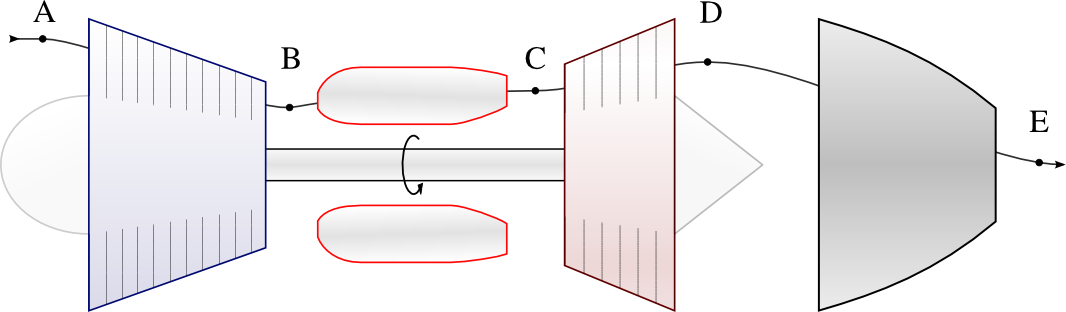
\includegraphics[width=\textwidth]{images/turbojet.png}
		\end{center}
		\caption{Schéma de principe d’un turboréacteur. L’air traverse la machine de gauche à droite.}
		\label{fig_exo_turbojet}
	\end{figure}
	
	Le moteur est testé sur un banc d’essai, à l’immobile. Lorsque l’air passe dans le turboréacteur, il traverse quatre composants que nous modéliserons comme s’ils étaient idéaux :
	
	\begin{description}
		\item [Le compresseur] comprime l’air de façon adiabatique réversible.\\
			À l’entrée, l’air est à \SI{0,9}{\bar} et \SI{5}{\degreeCelsius} ; à la sortie la pression est portée à \SI{19}{\bar}. 
		\item [La chambre de combustion] permet d’effectuer un réchauffement de l’air en maintenant sa pression constante.\\
			À la sortie de la chambre de combustion, la température est portée à \SI{1100}{\degreeCelsius}.
		\item [La turbine] extrait de l’énergie de l’air pour pouvoir alimenter le compresseur. Dans la turbine, l’air est détendu de façon adiabatique réversible.
		\item [La tuyère] est un composant dans lequel aucune puissance n’est apportée ou prélevée à l’air. Lorsqu’il la traverse, l’air se détend de façon adiabatique réversible ; sa vitesse augmente fortement. À la sortie de la tuyère, il a retrouvé la pression atmosphérique et est rejeté dans l’atmosphère.
	\end{description}
	
	Le but de l’exercice est de calculer la vitesse à laquelle le turboréacteur est capable de repousser l’air qu’il admet.
	
	\pagebreak[1] %handmade
	
	\begin{enumerate}
		\item À partir de la relation suivante,
			\begin{equation*}
				\left( \frac{p_1}{p_2} \right)	= \left( \frac{v_2}{v_1} \right)^{\gamma}
			\end{equation*}
							
			valable pour une évolution adiabatique réversible d’un gaz parfait, montrez (sans utiliser l’\cref{eq_isentropique_horrible1}) que :
			
			\begin{equation*}
				\left( \frac{T_1}{T_2} \right)	=  \left( \frac{p_1}{p_2} \right)^{\frac{\gamma -1}{\gamma}}
			\end{equation*}
			
		\item Quelle est la température de l’air à la sortie du compresseur ?
		\item Quelle est ainsi la puissance spécifique consommée par le compresseur ?
		\item Quelle est la puissance spécifique apportée sous forme de chaleur dans la chambre de combustion ?
		\item Quelle doit être la température à la sortie de la turbine pour qu’elle puisse alimenter le compresseur ?
		\item Quelle sera alors la pression à la sortie de la turbine ?
		\item Quelle sera la température des gaz d’échappement, à la sortie de la tuyère ?
		\item Quelle sera enfin la vitesse d’éjection des gaz à la sortie de la tuyère ?
		\item Tracez qualitativement l’évolution suivie par le gaz à travers le moteur sur un diagramme pression-volume.
		\item Sur le diagramme pression-volume plus haut, tracez qualitativement l’évolution qui serait suivie par le gaz si le compresseur ne pouvait pas effectuer une compression réversible (compresseur réel, compression avec frottement interne).
	\end{enumerate}


\exercisesolutionpage
\subsubsection*{Résultats}
	\linktosolutionsblurb

	\begin{description}
		\item [4.1] \tab 1) $\rho_1 = \SI{2,5}{\kilogram\per\metre\cubed}$; $v_1 = \SI{0,4}{\metre\cubed\per\kilogram}$ 
						\tab 2) $p_1 = \SI{2,103}{\bar}$
		\item [4.2] \tab $\Delta u = \SI{-536}{\kilo\joule\per\kilogram}$ (se calcule simplement avec la température finale)
		\item [4.3] \tab $w_{1\to 2} = \SI{+85,4}{\kilo\joule\per\kilogram}$ (\textsc{sfee} \& \ref{eq_h=cpT})
		\item [4.4] \tab 1) $m_1 = \SI{3,006}{\kilogram}$, $v_1 = \SI{0,3991}{\metre\cubed\per\kilogram}$, $\rho_1 = \SI{2,505}{\kilogram\per\metre\cubed}$, $p_1 = \SI{2}{\bar}$ ;
						\tab $m_2 = m_1$, $v_1 = v_2$, $\rho_1 = \rho_2$, $p_2 = \SI{2,395}{\bar}$.\\
						\tab 2) $m_{3} = \SI{2,51}{\kilogram}$, ainsi $m_\text{échap.} = \SI{0,4959}{\kilogram}$; 
						\tab 3) $p_4 = \SI{1,67}{\bar}$.
		\item [4.5] \tab 1) $w_\text{turbine} = \SI{-275}{\kilo\joule\per\kilogram}$ 	
						\tab 2) \SI{3,64}{\kilogram\per\second}
		\item [4.6] \tab 2) $w_{1 \to 2} = \SI{+257,58}{\kilo\joule\per\kilogram}$, $W_{1 \to 2} = \SI{+901,2}{\kilo\joule}$, $Q_{1 \to 2} = - W_{1 \to 2}$\\
					 	\tab 3) Oui, on aurait $v_{2 ad.} > v_{2 isoth.}$. 
		\item [4.7] \tab 2) $W_{1 \to 3} = \SI{+153,6}{\kilo\joule}$	
						\tab 3) $Q_{1 \to 3} = \SI{-625,3}{\kilo\joule}$
		\item [4.8] \tab Isotherme $2 \to 3$, isochore $1 \to 2$.
		\item [4.9] \tab \textit{Dans le sens horaire, en débutant à l’horizontale, sur les deux graphiques :} isobare ($p$~cste.), isotherme ($T$~cste.), adiabatique réversible, isochore ($v$~cst.).
		\item [4.10] 	\tab 2) $W_{B \to H} = \SI{+1,298}{\kilo\joule}$ 	
							\tab 3) $Q_{B \to H} = \SI{+0,3254}{\kilo\joule}$ 	
							\tab 4) \SI{1483,7}{\kelvin} 
							\tab 5) $S < \SI{3,164e-3}{\metre\squared}$
		\item [4.11] 	\tab 2) $\dot{W}_{1 \to 2} = \SI{+2,654}{\mega\watt}$ 	
							\tab 3) $T_{2b} = \SI{279,6}{\kelvin}$, $T_3 = \SI{752,6}{\kelvin}$, $\dot{W}_\text{comp. réel} = \SI{+3,726}{\mega\watt}$ (\SI{+40}{\percent})
		\item [4.12]	\tab 2) $T_2 = \SI{664,83}{\kelvin}$
							\tab 3) $w_\text{comp.} = \SI{+338,61}{\kilo\joule\per\kilogram}$
							\tab 4) $T_3 = \SI{1373,15}{\kelvin}$ ; ainsi $q_\text{comb} = \SI{+711,86}{\kilo\joule\per\kilogram}$
							\tab 5) $T_4 = \SI{986,47}{\kelvin}$
							\tab 6) $p_4 = \SI{5,97}{\bar}$
							\tab 7) $T_5 = \SI{574,49}{\kelvin}$
							\tab 8) $C_5 = \SI{909,98}{\metre\per\second}$\\
							\tab Bien sûr, ces valeurs ne tiennent pas compte des irréversibilités dans un turboréacteur réel. Ces effets sont étudiés dans le \coursdix.
	\end{description}
